\section{Static Pattern Classification on Real World Data}

Preprocessing came to be very essential in the dataset as the model operating on raw data was found to have very poor performance, with the occurrence of singular covariance matrices and with the EM maximization algorithm unable to converge properly with the sporadic changes in the log
likelihood. With further preprocessing, normalized data points were found to have increased classification accuracies. 

In the first attempt at preprocessing, columns 15 and 23 of the feature vectors were excluded(based on corresponding low eigenvalue obtained from the r matrix from q,r decomposition) which helped ameliorate the situation of singular covariance matrices during the algorithm run. The data was normalized vector wised and the following results were obtained with training accuracies peaking at 91 $\%$. However the use of Quantile transformation(non-parametric transformation which maps the input data onto a normal distribution ranging from 0 to 1) yielded the best results with classification accuracies in the order of 95$\%$, as this preprocessing technique is capable of reorganizing the data into normally distributed data(which is an underlying assumption of the GMM classifier) and also reducing the skewness of data which helps in eliminating the possibility of singular covariance matrices.


Dataset 2A consists of image histogram data pertaining to five class labels in which each image is represented by a 24 dimensional feature vector. The training accuracies were found to increase with increasing number of clusters in both cases. The best model was found to require much lower cluster numbers of gaussians in the case of full covariance matrix models compared to diagonal covariance matrix models. The full covariance matrix models were otherwise observed to perform poorly at higher cluster numbers as evident from the poorer performance on the validation data, unlike in the case of diagonal covariance matrix models. This can be perhaps attributed to the test data points lying outside the range of the gaussian basis functions as the models that operate on localised gaussian basis functions are not able to extrapolate to data points outside the range of the basis functions and therefore end up performing poorly on new unseen data points that lie much beyond the span of the gaussians. Further visual inspection of the images revealed that there were multiple types of images of the same type in the dev set, for instance in the case of coast images had multiple types which involved coast with sun, coast with only land,etc which may have interfered in the model functioning




% -----------------------------------------------------------
{\rowcolors{3}{green!40!yellow!10}{green!0!yellow!30}
\begin{table}[!h]
\centering
\begin{tabular}{ |c|c|c|  }
\hline
\rowcolor{lightgray} Model & Training Accuracy & Val Accuracy \\

[2,2,2,2,2] & 54.78$\%$  & 38.41$\%$ \\ 
\hline
[3,3,3,3,3] & 58.84$\%$  & 47.17$\%$ \\
\hline
[4,4,4,4,3] & 62.74$\%$  & 50.28$\%$ \\
\hline
[5,5,5,5,3] & 66.15$\%$  & 52.25$\%$ \\
\hline
[6,6,6,6,3] & 66.63$\%$  & 54.80$\%$ \\
\hline
\end{tabular}
\caption{Performance of models for Diagonal Covariance matrix with normalisation}.
\label{table:7}
\end{table}
}

% -----------------------------------------------------------
{\rowcolors{3}{green!40!yellow!10}{green!0!yellow!30}
\begin{table}[!h]
\centering
\begin{tabular}{ |c|c|c|  }
\hline
\rowcolor{lightgray} Model & Training Accuracy & Val Accuracy \\

[2,2,2,2,2] & 78.65$\%$  & 56.21$\%$ \\ 
\hline
[3,3,3,3,3] & 85.47$\%$  & 58.47$\%$ \\
\hline
[4,4,4,4,3] & 88.79$\%$  & 58.47$\%$ \\
\hline
[5,5,5,5,3] & 92.53$\%$  & 58.19$\%$ \\
\hline
[6,6,6,6,3] & 94.07$\%$  & 53.95$\%$ \\
\hline
\end{tabular}
\caption{Performance of models for Full Covariance matrix with normalisation}.
\label{table:7}
\end{table}
}

The best model was found by searching through all combinations of cluster parameters \ref{fig:27}, with the optimal model for diagonal covariance matrix model being [5,4,5,5,5], and the optimal model for full covariance matrix model being [3,3,4,5,2]


% -----------------------------------------------------------
{\rowcolors{3}{green!40!yellow!10}{green!0!yellow!30}
\begin{table}[!h]
\centering
\begin{tabular}{ |c|c|c|  }
\hline
\rowcolor{lightgray} Model & Training Accuracy & Val Accuracy \\
\hline
[1,1,1,1,1] & 23.71$\%$  & 22.88$\%$ \\   
 \hline
[2,2,2,2,2] & 33.69$\%$  & 25.42$\%$ \\ 
\hline
[3,3,3,3,3] & 41.48$\%$  & 26.84$\%$ \\
\hline
[4,4,4,4,4] & 50.48$\%$  & 34.46$\%$ \\
\hline
[5,5,5,5,5] & 55.27$\%$  & 37.56$\%$ \\
\hline
[6,6,6,6,6] & 57.14$\%$  & 37.85$\%$ \\
\hline
[6,5,6,6,4] & 55.11$\%$  & 39.54$\%$ \\
\hline
\end{tabular}
\caption{Performance of models for Diagonal Covariance matrix}.
\label{table:7}
\end{table}
}
\newpage
% -----------------------------------------------------------
{\rowcolors{3}{green!40!yellow!10}{green!0!yellow!30}
\begin{table}[!h]
\centering
\begin{tabular}{ |c|c|c|  }
\hline
\rowcolor{lightgray} Model & Training Accuracy & Val Accuracy \\
\hline
[1,1,1,1,1] & 74.84$\%$  & 56.21$\%$ \\   
 \hline
[2,2,2,2,2] & 85.63$\%$  & 55.36$\%$ \\ 
\hline
[3,3,3,3,3] & 90.67$\%$  & 54.51$\%$ \\
\hline
[4,4,4,4,4] & 94.72$\%$  & 52.25$\%$ \\
\hline
[5,5,5,5,5] & 97.56$\%$  & 46.32$\%$ \\
\hline
[6,6,6,6,6] & 98.37$\%$  & 41.24$\%$ \\
\hline
[3,3,4,5,2] & 93.58$\%$  & 58.75$\%$ \\
\hline
\end{tabular}
\caption{Performance of models for Full Covariance matrix}.
\label{table:8}
\end{table}
}

\begin{figure}[!ht]
    \centering
    \begin{subfigure}[t]{0.5\textwidth}
        \centering
        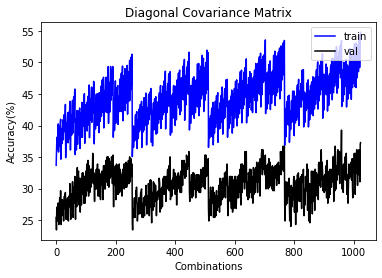
\includegraphics[height=2.5in]{Dataset_2a/diagonal covariance graph combinations.png}
        \caption{Diagonal covariance combinations}
    \end{subfigure}%
    ~ 
    \begin{subfigure}[t]{0.5\textwidth}
        \centering
        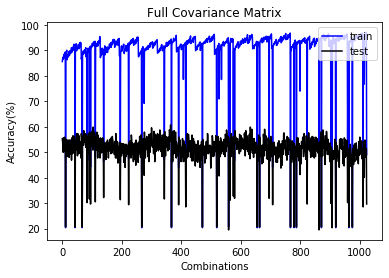
\includegraphics[height=2.5in]{Dataset_2a/full covariance graph combinations.png}
        \caption{Full covariance combinations}
    \end{subfigure}%
    ~
    \caption{Covariance Combinations}
    \label{fig:27}
\end{figure}

\newpage
\begin{figure}[!t]
    \centering
    \begin{subfigure}[t]{0.5\textwidth}
        \centering
        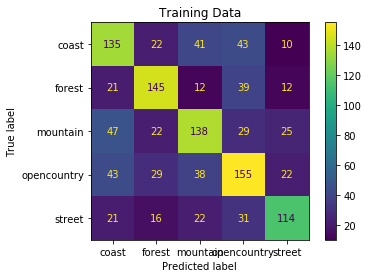
\includegraphics[height=2.5in]{Dataset_2a/diagonal covariance train confusion matrix.png}
        \caption{Train Data}
    \end{subfigure}%
    ~ 
    \begin{subfigure}[t]{0.5\textwidth}
        \centering
        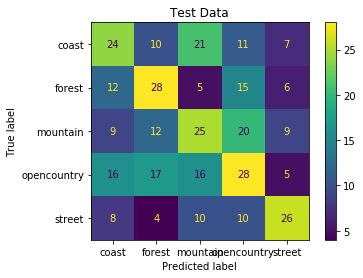
\includegraphics[height=2.5in]{Dataset_2a/diagonal covariance test confusion matrix.png} 
        \caption{Validation Data}
    \end{subfigure}%
    ~
    \caption{Confusion Matrix for diagonal covariance}
    \label{fig:28}
\end{figure}

\newpage
\begin{figure}[!h]
    \centering
    \begin{subfigure}[t]{0.5\textwidth}
        \centering
        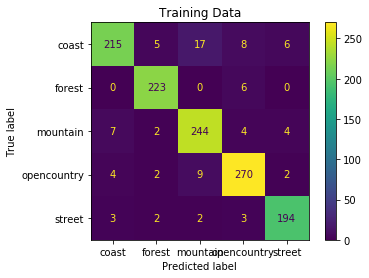
\includegraphics[height=2.5in]{Dataset_2a/full covariance train confusion matrix.png} 
        \caption{Train Data}
    \end{subfigure}%
    ~ 
    \begin{subfigure}[t]{0.5\textwidth}
        \centering
        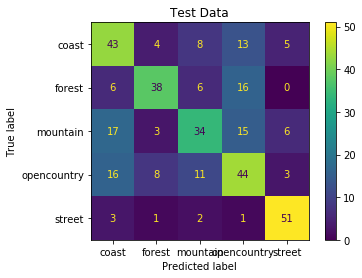
\includegraphics[height=2.5in]{Dataset_2a/full covariance test confusion matrix.png}
        \caption{Validation Data}
    \end{subfigure}%
    ~
    \caption{Confusion Matrix for full covariance}
    \label{fig:29}
\end{figure}

\section{Varying Length Pattern Classification for Real World Data}


Dataset 2B consists of image histogram data pertaining to five class labels in which each image is represented by a set of 36, 23 dimensional vectors, i.e each image is represented by $36x23$ matrix. In the training phase each of row from the image matrices are treated as separate examples with the
same label as the parent image. In the classification phase, the classification of each image involves the calculating of the conditional probability that the image belongs to the class i as the product of the individual conditional probabilities of its constituent rows, i.e for an image matrix X and class label i.

 \begin{align*}
      p(y=y_i) &= \prod_{n=1}^{n} p(y=y_i) \\
                    &= \prod_{j=1}^{N}\sum_{k=1}^{K}w_{ik}. \mathcal{N}(x_n|\mu_{ik},c_{ik})
  \end{align*}
  

In both cases, the optimal model was found to be the cluster combination of [8,8,8,8,8] and a thorough search through the combination parameters were not feasible as the training of the model is computationally expensive across 150,000 data points

% -----------------------------------------------------------
{\rowcolors{3}{green!40!yellow!10}{green!0!yellow!30}
\begin{table}[!h]
\centering
\begin{tabular}{ |c|c|c|  }
\hline
\rowcolor{lightgray} Model & Training Accuracy & Val Accuracy \\
\hline
[1,1,1,1,1] & 23.13$\%$  & 22.88$\%$ \\   
 \hline
[2,2,2,2,2] & 45.77$\%$  & 47.17$\%$ \\ 
\hline
[3,3,3,3,3] & 57.62$\%$  & 47.45$\%$ \\
\hline
[4,4,4,4,4] & 61.85$\%$  & 51.97$\%$ \\
\hline
[5,5,5,5,5] & 67.37$\%$  & 61.58$\%$ \\
\hline
[6,6,6,6,6] & 69.64$\%$  & 62.42$\%$ \\
\hline
[7,7,7,7,7] & 70.21$\%$  & 66.10$\%$ \\
\hline
[8,8,8,8,8](optimal)  & 73.62 $\%$  & 66.66 $\%$ \\
\hline
\end{tabular}
\caption{Performance of models for Diagonal Covariance matrix}.
\label{table:9}
\end{table}
}

% -----------------------------------------------------------
{\rowcolors{3}{green!40!yellow!10}{green!0!yellow!30}
\begin{table}[!ht]
\centering
\begin{tabular}{ |c|c|c|  }
\hline
\rowcolor{lightgray} Model & Training Accuracy & Val Accuracy \\
\hline
[1,1,1,1,1] & 88.39$\%$  & 83.61$\%$ \\   
 \hline
[2,2,2,2,2] & 94.80$\%$  & 80.50$\%$ \\ 
\hline
[3,3,3,3,3] & 95.86$\%$  & 85.31$\%$ \\
\hline
[4,4,4,4,4] & 97.40$\%$  &  90.67 $\%$ \\
\hline
[5,5,5,5,5] & 98.86$\%$  & 94.63$\%$ \\
\hline
[6,6,6,6,6] & 99.02$\%$  & 94.63$\%$ \\
\hline
[7,7,7,7,7] & 99.26$\%$  & 94.35$\%$ \\
\hline
[8,8,8,8,8](optimal)  &  99.67 $\%$  & 95.19 $\%$ \\
\hline
\end{tabular}
\caption{Performance of models for Full Covariance matrix}.
\label{table:10}
\end{table}
}
\newpage




%------------------------------------------------------------
% \subsubsection*{Model Accuracy across combinations}

% \begin{figure}[!ht]
%     \centering
%     \begin{subfigure}[t]{0.5\textwidth}
%         \centering
%         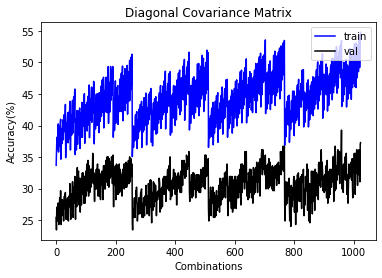
\includegraphics[height=2.5in]{Dataset_2a/diagonal covariance graph combinations.png}
%         \caption{Diagonal covariance combinations}
%     \end{subfigure}%
%     ~ 
%     \begin{subfigure}[t]{0.5\textwidth}
%         \centering
%         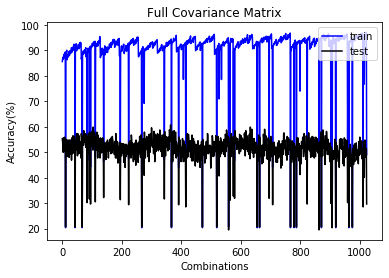
\includegraphics[height=2.5in]{Dataset_2a/full covariance graph combinations.png}
%         \caption{Full covariance combinations}
%     \end{subfigure}%
%     ~
%     \caption{Covariance Combinations}
%     \label{fig:23}
% \end{figure}


\begin{figure}[!h]
    \centering
    \begin{subfigure}[t]{0.5\textwidth}
        \centering
        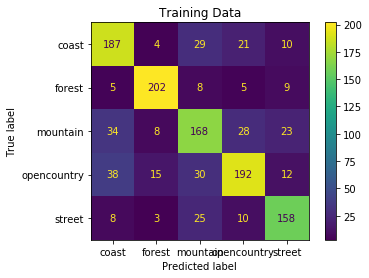
\includegraphics[height=2.5in]{Dataset_2b/diagonal covariance train confusion matrix.png}
        \caption{Train Data}
    \end{subfigure}%
    ~ 
    \begin{subfigure}[t]{0.5\textwidth}
        \centering
        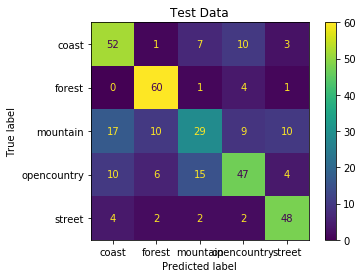
\includegraphics[height=2.5in]{Dataset_2b/diagonal covariance test confusion matrix.png}
        \caption{Validation Data}
    \end{subfigure}%
    ~
    \caption{Confusion Matrix for diagonal covariance}
    \label{fig:30}
\end{figure}

%------------------------------------------------------------
%\newpage

\begin{figure}[!h]
    \centering
    \begin{subfigure}[t]{0.5\textwidth}
        \centering
        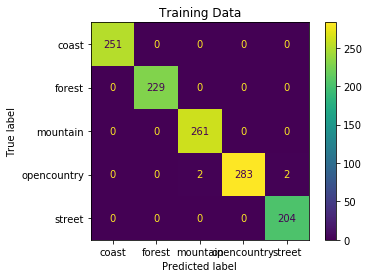
\includegraphics[height=2.5in]{Dataset_2b/full covariance train confusion matrix.png} 
        \caption{Train Data}
    \end{subfigure}%
    ~ 
    \begin{subfigure}[t]{0.5\textwidth}
        \centering
        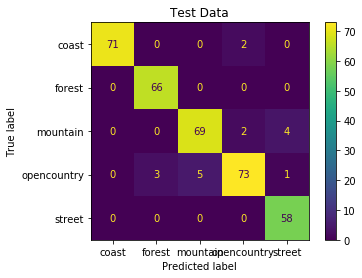
\includegraphics[height=2.5in]{Dataset_2b/full covariance test confusion matrix.png}
        \caption{Validation Data}
    \end{subfigure}%
    ~
    \caption{Confusion Matrix for full covariance}
    \label{fig:31}
\end{figure}